
\chapter[Contexto do Negócio]{Contexto do Negócio}
\section{Introdução}
A organização FGRacing é uma equipe de competição da Universidade de Brasília -
Campus Gama. Atualmente, seu principal projeto é o desenvolvimento e construção
de um veículo Fórmula SAE elétrico. Este é um veículo especial para a competição
Fórmula SAE Brasil, e um protótipo dele pode ser observado na figura \ref{sae}.

\begin{figure}[!h]
        \centering
        \includegraphics[keepaspectratio=true,scale=0.3]{figuras/sae.eps}
        \caption{Protótipo - Fórmula SAE\label{sae}}
\end{figure}

A equipe é organizada de forma vertical, seguindo a seguinte ordem de hierarquia:

\begin{itemize}
  \item Capitania;
  \item Gerência de projetos;
  \item Líderes de Equipe (Membros os quais gerenciam os setores da empresa (times));
  \item Membros de Equipe.
\end{itemize}

A Capitania é o nível mais alto da Equipe. O Capitão é responsável por tomar as decisões estratégicas da equipe e decidir o que será realizado pelas equipes.

As equipes da FGR são divididas em duas frentes principais: Administrativo e Operacional. Cada uma dessas frentes é administrada por um Gerente de Projeto, que é responsável por gerenciar as equipes e delegar, revisar e validar atividades a cada uma delas.

O Líder de Equipe é responsável por cumprir as atividades delegadas pelo gerente de projeto, gerenciando a equipe e delegando tarefas para cada membro de equipe.

Já o Membro de equipe é responsável por executar e produzir relatórios sobre as tarefas delegadas pelo Líder da sua equipe.

É importante ressaltar que, nesta organização, o mesmo indivíduo pode exercer mais de um papel na equipe, um em cada frente da FGR. Por exemplo, um membro da equipe de Marketing, contida na Frente Administrativa, pode, ao mesmo tempo, ser Líder da equipe de Estruturas, contida na Frente Operacional da organização.

\section{Elicitação de Requisitos}

Visando o pleno entendimento do contexto e problemas da equipe, bem como coletar os requisitos do sistema de
maneira satisfatória, foi definida a aplicação de três técnicas de elicitação de requisitos, como foi descrito no
relatório anterior do projeto: Entrevista, Brainstorming e Observação.

A aplicação destas técnicas possibilitou a compreensão dos gargalos presentes no processo utilizado pela organização e a
elaboração de uma solução de software que auxilie na resolução destes obstáculos.

A técnica de Observação foi aplicada por meio do acompanhamento das atividades da FGR em suas ferramentas de comunicação e
organização de arquivos, e em suas Reuniões Gerais.

A equipe de Analistas de Requisitos observou e avaliou o uso da ferramenta de comunicação \textit{“WhatsApp”} e da ferramenta de
arquivamento em nuvem \textit{“Google Drive”} por parte dos membros da organização. Esta observação resultou em uma compreensão da
maneira como a equipe trabalha, se comunica e se organiza, o que possibilitou a identificação de problemas. Além disso, o
acompanhamento das Reuniões Gerais quinzenais da equipe revelou que os times possuem uma baixa visibilidade da totalidade
da equipe. A inexistência da prática de documentação das reuniões também é um fator que gera problemas.

A técnica de Entrevista foi realizada na modalidade de “Entrevista Fechada”, que consiste em uma reunião, onde o analista
de requisitos submete um stakeholder a uma série de perguntas pré-definidas \cite{gunda2008}. O roteiro da entrevista realizada
pode ser encontrado no anexo \ref{annex:roteiro}.

A Entrevista foi aplicada pela equipe de análise de requisitos a dois membros da FGRacing. As respostas foram documentadas
e analisadas pela equipe, o que resultou em um conhecimento mais aprofundado do contexto, do processo e das dificuldades
enfrentadas pela equipe. A ata da reunião onde a entrevista foi realizada pode ser encontrada no apêndice \ref{appendix:reuniao1}.

O Brainstorming consiste em uma técnica de grupo utilizada para gerar soluções para um problema específico \cite{gunda2008}.
Esta técnica foi aplicada por meio de uma reunião com stakeholders. Por causa de compromissos imprevistos, a presença de
membros da FGR nesta reunião não foi possível. Apesar disto, a reunião não pôde ser adiada, pois isto resultaria em um
atraso muito grande no andamento do projeto. Por isso, o Brainstorming foi realizado apenas pelos quatro membros da equipe
de desenvolvimento.

As propostas para solução de software para a FGRacing, geradas no Brainstorming, foram apresentadas para o cliente, após
serem concluídas, para que fossem validadas. Esta prática possibilitou a aplicação adequada da técnica, mesmo sem a presença
 do cliente, o que evitou atrasos ou a elicitação incorreta de requisitos.





\section{Problema}
Apesar da organização, a equipe enfrenta dificuldades na gerência dos projetos realizados. A integração entre os setores é falha,
 pois não existe uma comunicação eficiente entre eles. A falha na comunicação faz com que os membros sintam-se desmotivados,
  visto que a má integração das áreas causa a sensação de que o projeto está estagnado. Como consequência da desmotivação,
  os membros atrasam as tarefas, comprometendo o projeto, enquanto outros chegam a abandonar a equipe.

A empresa já tentou utilizar ferramentas de auxílio de gerência, porém a maioria não obteve sucesso. Entre elas pode-se
 citar: Trello, Slack, Whatsapp, Facebook e Google Drive. Dentre essas ferramentas, as únicas quem ainda se encontram
 em utilização são o Whatsapp e Google Drive. Quanto as que tiveram seu uso parado foram relatadas os seguintes problemas:

\begin{itemize}
  \item \textbf{Trello:} os líderes designavam atividades e tarefas para seus membros do setor , mas não davam feedback sobre suas execuções.
  \item \textbf{Slack:} os membros mostram muita resistência em migrar e se adaptar à nova plataforma.
  \item \textbf{Facebook:} utilizado apenas 2 vezes para fazer enquetes com a equipe.
\end{itemize}

Uma consequência da utilização de muitas ferramentas é a descentralização de informações. Isto torna árduo o controle de
informações, visto que não há padronização da divulgação destas, o que causa retrabalho na busca e compartilhamento da notícia
ou arquivo desejado.

O armazenamento de  documentos, .CADs e outros arquivos, é feito através do Google Drive. Entretanto, o compartilhamento de
 um arquivo nessa plataforma acaba sendo entre todos os membros da equipe, de forma que todos os membros têm acesso à
 documento que seriam “privados” de um setor específico. Isso acarreta numa falha de segurança: membros podem modificar, e
  até mesmo deletar, mesmo que não-intencionalmente, arquivos privados e cruciais para o projeto. Até mesmo usuários mal
  intencionados poderiam prejudicar a Equipe, ainda que não haja relatos desse tipo de experiência.

Outro ponto em que a equipe falha é no desenvolvimento de documentação interna, especialmente em atas de reuniões e documentos
 técnicos sobre o projeto. A consequência da ausência de documentação sobre as reuniões são: informações perdidas, tomadas
  de decisões erradas, o que de certo modo faz com as reuniões acabem não tendo um cunho oficial. Os documentos técnicos,
  por sua vez, são, geralmente, feitos tardiamente, apenas quando necessários. Isto prejudica a equipe principalmente em
  momentos em que é necessário apresentar o projeto para algum potencial patrocinador.

A gerência da FGRancing vem até então demonstrando dificuldades em administrar a equipe com as ferramentas já dispostas
 no mercado. Nesse cenário, se faz necessário a elaboração de um software que atenda às peculiaridades	administrativas
  da empresa.

  \pagebreak
\subsection{Diagrama de Causa e Efeito (Fishbone)}
Com a finalidade de traçar os sub-problemas e que levam a raiz do problema, a Equipe de Engenharia de Requisitos, em conjunto com o cliente, elaborou um Diagrama de Causa e Efeito (Fishbone). Este diagrama, evoluído e priorizado com a professora e o cliente, permitiu evidenciar as raízes do problema maior da empresa: a falha na comunicação e transparência da equipe.

A representação gráfica deste diagrama é apresentada na Figura \ref{fishbone}.

\begin{figure}[!h]
        \centering
        \includegraphics[keepaspectratio=true,scale=0.9]{figuras/fishbone.eps}
        \caption{Diagrama de Fishbone\label{fishbone}}
\end{figure}


\subsection{Resumo da Solução}
A solução proposta proposta foi o desenvolvimento de uma plataforma web  capaz de integrar a gerência de atividades, pessoas e arquivos.
Esta solução foi denominada \textbf{AutoTrack} e está brevemente explicitada a seguir.

\subsection{Feed de Atividades}
A ferramenta irá dispor de um feed de atividades, onde todos os membros da equipe poderão visualizar o andamento
 dos projetos através do acompanhamento das ações realizadas. A ferramenta será capaz, ainda, de gerar
  relatórios automatizados sobre o status das atividades.

\subsection{Estrutura de Kanbans}
O sistema irá dispor de um esquema de kanbans estruturados conforme a hierarquia da empresa. O capitão poderá designar tarefas para os times,
bem como acompanhar seu desenvolvimento. Os líderes de setores, por sua vez, receberão as atividades a eles designadas,
 e distribuirão aos seus membros. Por fim, o time utiliza o kanban para organizar e informar a rastreabilidade das tarefas.

\subsection{Gerência de Arquivos e Documentos}
A entrega de uma atividade pode ser dependente da anexação de um arquivo. O sistema AutoTrack irá
gerenciar estes anexos, organizando-os conforme os setores da equipe, e suas áreas. Os arquivos terão um nível de privacidade.
 Assim, arquivos de setores específicos ficarão disponíveis para modificações apenas para membros deste setor, porém
  ficarão disponíveis para os membros de outros setores apenas para visualização.


%%%%%%%%%%%%%%%%%%%%%%%%%%%%
\chapter{Gerência de Requisitos}
\section{Nível de Portfólio}
O nível de portfólio é a camada do SAFe que proporciona uma visão com maior abstração, permitindo a identificação dos temas de investimento
do projeto e por consequência, os épicos. O nosso processo apresenta as seguintes atividades no nível de portfólio:

\begin{itemize}
  \item Analisar e entender o contexto da FGR;
  \item Definir épicos;
  \item Analisar e priorizar épicos
  \item Validar e administrar mudanças
\end{itemize}

\pagebreak

\begin{figure}[!h]
        \centering
        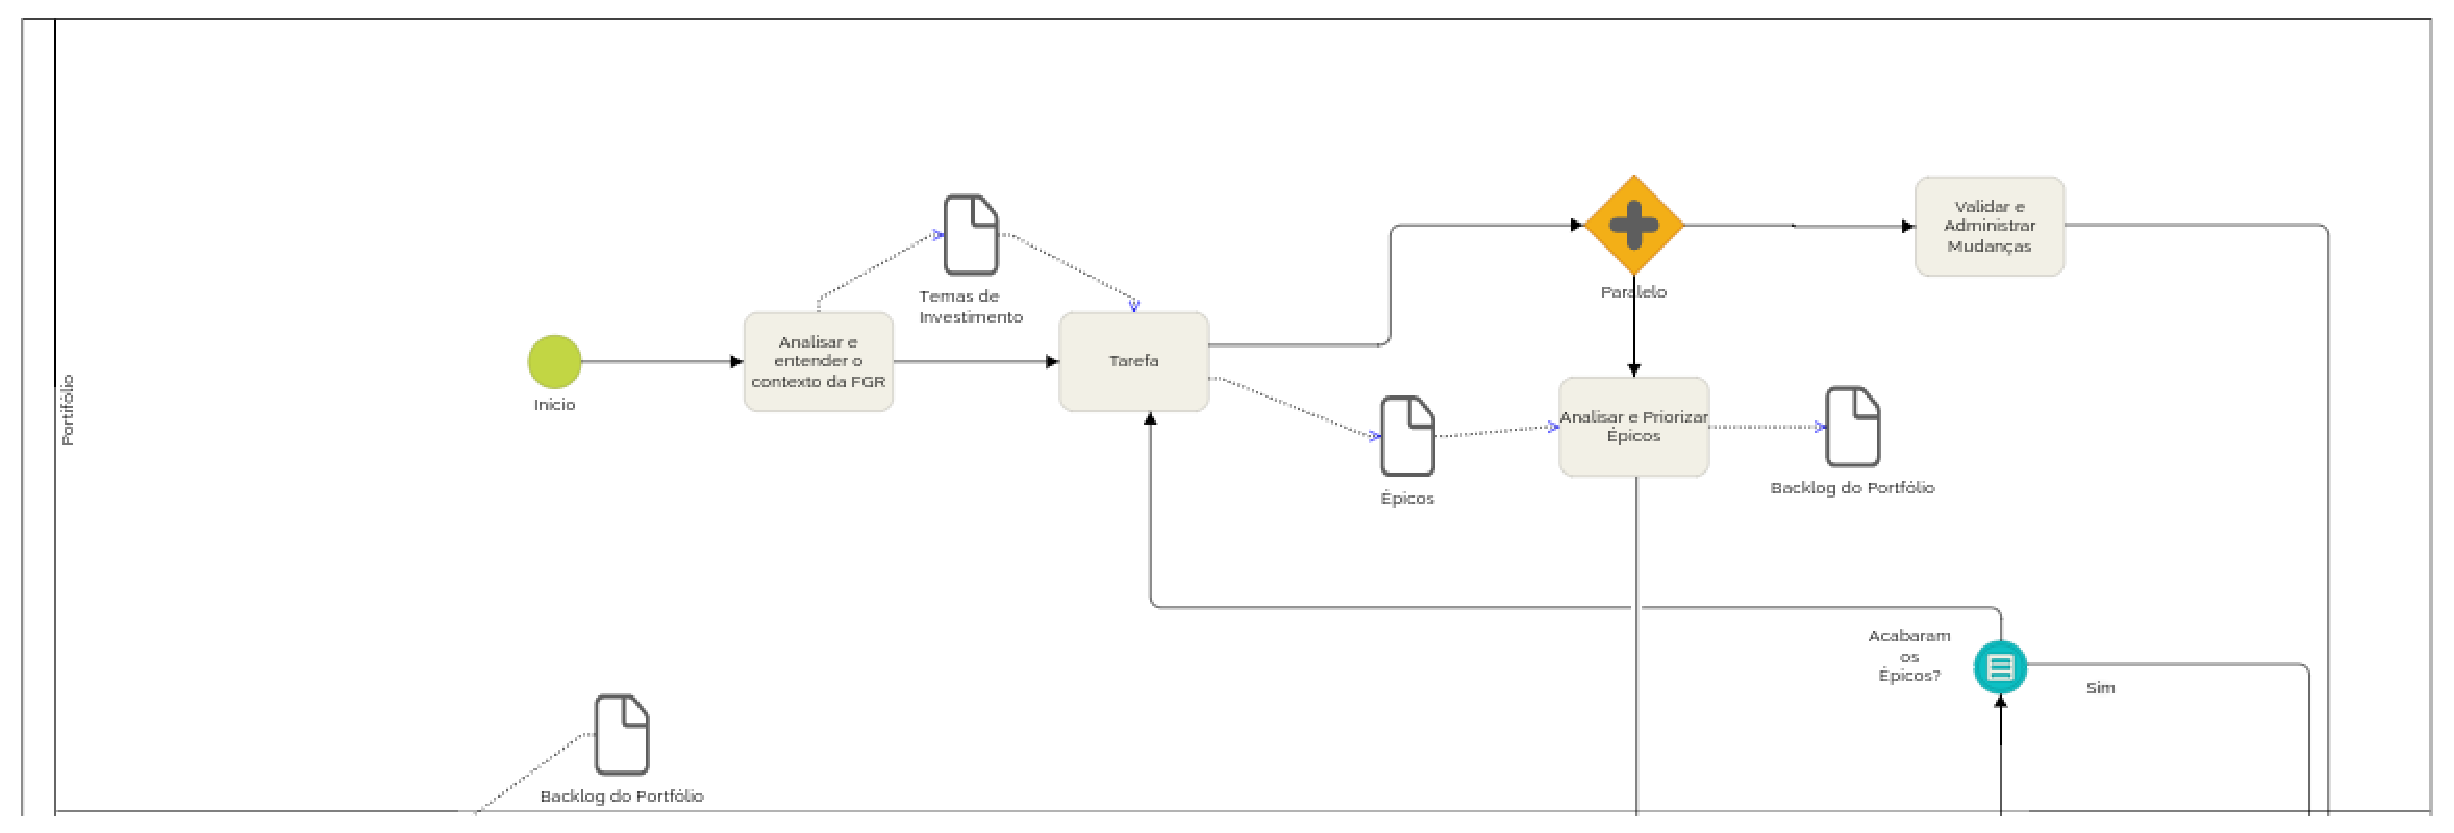
\includegraphics[keepaspectratio=true,scale=0.42]{figuras/prog.eps}
        \caption{Processo a nível de Portfólio}
\end{figure}

O cumprimento das tarefas listadas se deu por meio das técnicas de elicitação de requisitos presentes no T1,
 brainstorming e entrevistas.

\subsection{Backlog do Portfólio}

Após analisar e entender o contexto da FGR identificou-se que havia necessidade na equipe de uma melhoria na comunicação
 e na transparência das atividades, o que se revelou em tema de investimento e também problema central identificado pela
  ferramenta diagrama de causa e efeito. Desse tema de investimento derivaram-se os seguintes épicos:

\begin{itemize}
  \item \textbf{Épico 01 - EP-01:} \textit{Gerenciamento de Atividades:} Contempla a estruturação dos kanbans e a visualização das atividades realizadas pelos diferentes grupos da empresa.
  \item \textbf{Épico 02 - EP-02:} \textit{Gerenciamento de Pessoas:} Abrange todas as ações de cadastro e administração de pessoas por parte do sistema.
  \item \textbf{Épico 03 - EP-03:} \textit{Gerenciamento de Arquivos e Permissões:} Envolve o controle de acesso a documentos da equipe em diferentes grupos.
  \item \textbf{Épico 04 - EP-04:} \textit{Gerar Relatórios Automatizados:} Diz respeito a automatização de relatórios para somar à documentação da empresa.
\end{itemize}


\subsection{Roadmap}
Roadmap é uma técnica flexível amplamente utilizada na indústria para apoiar o planejamento estratégico e a longo
alcance \cite{phaal}. O roadmap fornece um meio para melhorar o "radar" de uma empresa, expandindo seus horizontes de
planejamento, juntamente com a identificação e avaliação de possíveis ameaças e oportunidades no ambiente de negócios.

Segundo o SAFe \cite{safe}, esta técnica fornece uma espécie de plano do que está e do que será feito na empresa ou organização.
No contexto de um roadmap os times sabem quais seus compromissos, bem como qual o plano de intenções futuras. O roadmap
relaciona entregas planejadas com unidades de tempo.

Neste projeto, o roadmap foi produzido de forma que features não-interdependentes pudessem ser elaboradas paralelamente, de
forma a atender as demandas de prioridade sugeridas pelo usuário, sem comprometer o desenvolvimento adequado. A figura a
seguir apresenta o Roadmap priorizado, para o espaço de tempo da disciplina.

\begin{figure}[!h]
        \centering
        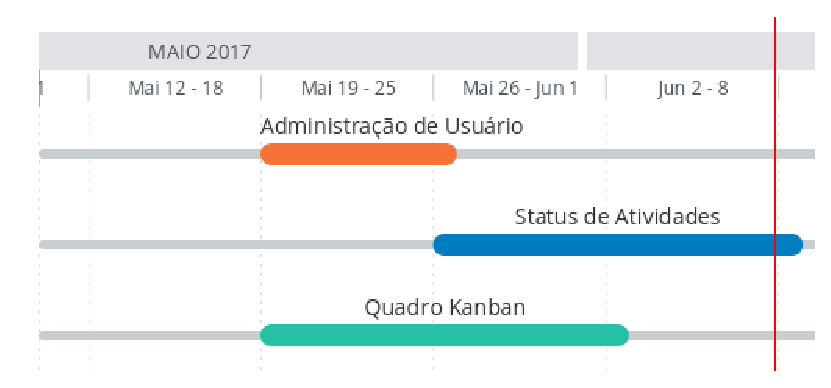
\includegraphics[keepaspectratio=true,scale=0.8]{figuras/roadm.eps}
        \caption{Roadmap - PI 1}
\end{figure}

O anexo \ref{annex:roadmap} apresenta, integralmente, o Roadmap proposto para todo o projeto.
